% to copy from the backup section of federated_learning_optim.tex
\begin{document}

%----------------------------------------------------------------------------------------
%	TITLE PAGE
%----------------------------------------------------------------------------------------

\title[Personalization]{Talk 4: Personalization in Federated Learning --- II}
\date{2021年6月10日}
\author[]{WEN Hao}

% \institute[北京航空航天大学] % Your institution as it will appear on the bottom of every slide, may be shorthand to save space
% {
% 数学科学学院 \\ % Your institution for the title page
% \medskip
% \textit{wenh06@gmail.com} % Your email address
% 北京航空航天大学 \\
% 数学科学学院 \qquad 北京航空航天大学
% }

% \logo{\includegraphics[height=1.5cm]{logo}}
% \logoii{\includegraphics[height=1cm]{logo2}}

% \date{\footnotesize 2021年4月13日} % Date, can be changed to a custom date

\setlength{\belowdisplayskip}{5pt} \setlength{\belowdisplayshortskip}{5pt}
\setlength{\abovedisplayskip}{5pt} \setlength{\abovedisplayshortskip}{5pt}

%------------------------------------------------

\begin{frame}
\titlepage % Print the title page as the first slide
\end{frame}

\begin{frame}
\frametitle{Personalization for FL}

{\bfseries When does one need personalization?}

\vspace{0.2em}
\noindent --- When data across clients are ``enough'' non-IID, which is more realistic.

\pause
\vspace{0.8em}

{\bfseries Means of personalization:}
\begin{itemize}
    \item Federated Multi-Task Learning (+ regularization / proximal term), e.g. \cite{smith2017mocha}
    \item Model-Agnostic Meta Learning, e.g. \cite{finn2017maml}
    \item Local Fine-tuning.
    \item etc.
\end{itemize}

\end{frame}

%------------------------------------------------

\section[MAML]{Model-Agnostic Meta Learning}

%------------------------------------------------
% Page 15

\begin{frame}
\frametitle{Model-Agnostic Meta Learning}

\begin{quote}
    ``The goal of meta-learning is to train a model on a {\bfseries variety of {\color{red} learning tasks}}, such that it can solve new learning tasks using only a small number of training samples.'' \hfill -- \cite{finn2017maml}
\end{quote}

\vspace{0.6em}

i.e. over a distribution of learning tasks $p(\mathcal{T})$, where
$$\mathcal{T} = \{ \mathcal{L}(\{(x_t,a_t)\}), q(x_1), q(x_{t+1}|x_t, a_t), H \}$$
with
\begin{align*}
    & (x_t,a_t): & \text{data points} \\
    & \mathcal{L}: & \text{loss function} \\
    & q(x_1): & \text{initial distribution} \\
    & q(x_{t+1}|x_t, a_t): & \text{transition} \\
    & H: & \text{episode length}
\end{align*}

\end{frame}

%------------------------------------------------
% Page 15

\begin{frame}
\frametitle{Model-Agnostic Meta Learning}

\begin{block}{Intuition of MAML}
Some internal representations are more transferrable than others. MAML should encourage the emergence of such general-purpose representations via searching for model parameters that are sensitive to changes in the task.
\end{block}

\begin{figure}
    \centering
    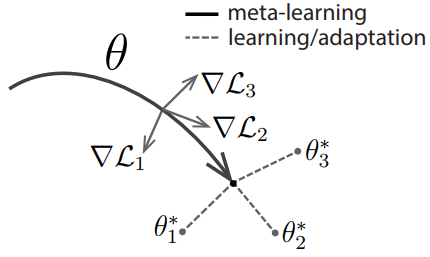
\includegraphics[keepaspectratio,width=.7\textwidth]{images/maml.png}
    \label{fig:my_label}
\end{figure}

\end{frame}

%------------------------------------------------
% Page 15

\begin{frame}
\frametitle{Model-Agnostic Meta Learning}

\begin{algorithm}[H]
\SetAlgoNoLine
\DontPrintSemicolon
{\bfseries Require:} $p(\mathcal{T})$ distribution over tasks\;
{\bfseries Require:} $\alpha, \beta$ step size hyper-params\;
randomly initialize model params $\theta$\;
\While{not done}{
    Sample batch of tasks $\mathcal{T}_i \sim p(\mathcal{T})$\;
    \For{all $\mathcal{T}_i$}{
        Evaluate $\nabla_{\theta} \mathcal{L}_{\mathcal{T}_i}(f_{\theta})$ w.r.t. $K$ samples\;
        Compute adapted parameters with gradient descent $\theta'_i = \theta - \alpha \nabla_{\theta} \mathcal{L}_{\mathcal{T}_i}(f_{\theta})$\;
    }
    Update \colorbox{pink}{$\theta \leftarrow \theta - \beta \nabla_{\theta} \sum\limits_{\mathcal{T}_i\sim p(\mathcal{T})} \mathcal{L}_{\mathcal{T}_i} (f_{\theta_i'})$} (gradient through gradients)\;
}
\caption{MAML\cite{finn2017maml}}
\end{algorithm}

\end{frame}

%------------------------------------------------
% Page 15

\begin{frame}

to update....

\end{frame}

%------------------------------------------------

\section[FMTL]{Federated Multi-Task Learning}

%------------------------------------------------
% Page 15

\begin{frame}
\frametitle{Federated Multi-Task Learning}

\begin{itemize}
    \pgfsetfillopacity{0.4}
    \item Mixture of global and local \cite{hanzely2020federated}:
    $$\text{minimize} \quad \sum\limits_{i=1}^N f_i(x_i) + \dfrac{\lambda}{2} \sum\limits_{i=1}^N \lVert x_i - {\color{red} \overline{x}} \rVert^2$$
    \pgfsetfillopacity{1}
    \item pFedMe (bi-level) \cite{t2020pfedme} (and similarly EASGD\cite{zhang2015easgd}):
    \begin{align*}
        & \text{minimize} \quad \sum\limits_{i=1}^N F_i(x), \\
        & \text{where} \quad F_i(x) = \min \left\{ f_i(x_i) + \dfrac{\lambda}{2} \lVert x_i - {\color{red} x}\rVert^2 \right\}
    \end{align*}
    \item FedU \cite{dinh2021fedu}:
    $$\text{minimize} \quad \sum\limits_{i=1}^N f_i(x_i) + \dfrac{\lambda}{2} \sum\limits_{i=1}^N {\color{red} \sum\limits_{j\in\mathcal{N}_i}} \lVert x_i - {\color{red} x_j} \rVert^2$$
\end{itemize}

\end{frame}

%------------------------------------------------
% Page 15

\begin{frame}
\frametitle{pFedMe}

to update....

\end{frame}

%------------------------------------------------
% Page 15

\begin{frame}

to update....

\end{frame}

%------------------------------------------------
% Page 15

\begin{frame}

to update....

\end{frame}

%------------------------------------------------
% Page 15

\begin{frame}

to update....

\end{frame}

%------------------------------------------------
% Page 15

\begin{frame}

to update....

\end{frame}

%------------------------------------------------
% Page 15

\begin{frame}

to update....

\end{frame}

%------------------------------------------------
% Page 15

\begin{frame}

to update....

\end{frame}

%------------------------------------------------
% Page 15

\begin{frame}[allowframebreaks]
\frametitle{参考文献}

{\footnotesize
\bibliographystyle{ieeetr}
\bibliography{references}
}

\end{frame}

%------------------------------------------------

\end{document}